\begin{problem}[3]
    $5x^2 + 6xy + 5y^2 - 4\sqrt{2}x + 4\sqrt{2}y = 0$
\end{problem}

\begin{solution}[Solution]
    First things first let's analyze our first three coefficients. 
    
    \[ \boxed{A = 5} \; \boxed{B = 6} \; \boxed{C = 5} \]
    
    \begin{align}
        B^2 - 4 \cdot A \cdot C & \\
        6^6 - (4 \cdot 5 \cdot 5) & \\
        36 - 100 &< 0
    \end{align}
    
    Our answer being less than 0 implies that our answer will either be an ellipse or a circle. Next we need to ascertain how rotated our plot will be.
    
    \begin{align}
        cot(2\theta) &= \frac{A - C}{B} \\
        cot(2\theta) &= \frac{5-5}{6} \\
        cot(2\theta) &= 0 \\
        cot(\theta) &= 0 \; \text{when} \; \theta = \frac{\pi}{2} \\
        2\theta &= \frac{\pi}{2} \\
        \theta &= \frac{\pi}{4} + \frac{\pi}{2}k \; \text{for any integer k}
    \end{align}
    
    How convenient, it's the same as the last problem. This actually has huge implications for the state of my sanity. This means we can skip calculating $x$, $y$, $x^2$, $y^2$ and $xy$ because we're working with the same angle as last time. For the sake of clarity though let me just list the final results of those calculations below.
    
    \[\boxed{x = \frac{x' \cdot \sqrt{2}}{2} - \frac{y' \cdot \sqrt{2}}{2}}\]
    
    \[\boxed{y = \frac{x' \cdot \sqrt{2}}{2} + \frac{y' \cdot \sqrt{2}}{2}}\]
    
    \[\boxed{x^2 = \frac{(x')^2}{2} - \frac{(2\cdot (x' \sqrt{2})) \cdot (2 \cdot (y' \sqrt{2}))}{4} + \frac{(y')^2}{2}}\]
    
    \[\boxed{y^2 = \frac{(x')^2}{2} + \frac{(2\cdot (x' \sqrt{2})) \cdot (2 \cdot (y' \sqrt{2}))}{4} + \frac{(y')^2}{2}}\]
    
    \[\boxed{xy = \frac{(x')^2}{2} - \frac{(y')^2}{2}}\]
    
    From here we're back at the spicy bit, we need to place all of these back into our given equation. It'll be mostly the same as last time, but with different coefficients. We'll see how it works out! 
    
    \begin{align}
        0 &= 5x^2 + 6xy + 5y^2 - 4\sqrt{2}x + 4\sqrt{2}y \\
        0 &= \left( 5 \cdot \left( \frac{(x')^2}{2} - \frac{(2\cdot (x' \sqrt{2})) \cdot (2 \cdot (y' \sqrt{2}))}{4} + \frac{(y')^2}{2} \right) \right) + \left( 6 \cdot \left( \frac{(x')^2}{2} - \frac{(y')^2}{2} \right) \right) + \\ 
        & \left( 5 \cdot \left( \frac{(x')^2}{2} + \frac{(2\cdot (x' \sqrt{2})) \cdot (2 \cdot (y' \sqrt{2}))}{4} + \frac{(y')^2}{2} \right) \right) - \left( \left( \frac{x' \cdot \sqrt{2}}{2} - \frac{y' \cdot \sqrt{2}}{2} \right) \cdot 4\sqrt{2} \right) + \\
        & \left( \left( \frac{x' \cdot \sqrt{2}}{2} + \frac{y' \cdot \sqrt{2}}{2} \right) \cdot 4\sqrt{2} \right) 
    \end{align}
    
    Alright, here we go. We'll break this into chunks again and simplify from there. First we'll start with the two largest chunks, 1 and 3. \medskip
    
    Chunks 1 \& 3:
    
    \begin{align}
        \text{Chunks 1 and 3} &= \frac{5(x')^2}{2} - \frac{(5\cdot (x' \sqrt{2})) \cdot (5 \cdot (y' \sqrt{2}))}{4} + \frac{5(y')^2}{2}  + \\
        & \frac{5(x')^2}{2} + \frac{(5\cdot (x' \sqrt{2})) \cdot (5 \cdot (y' \sqrt{2}))}{4} + \frac{5(y')^2}{2} \\
        &= \frac{10(x')^2}{2} + \frac{10(y')^2}{2}
    \end{align}
    \[\boxed{\text{Chunks 1 and 3} = 5(x')^2 + 5(y')^2}\]
    
    Chunk 2:
    
    \[\text{Chunk 2} = \left( 6 \cdot \left( \frac{(x')^2}{2} - \frac{(y')^2}{2} \right) \right)\]
    \[\boxed{\text{Chunk 2} = 3(x')^2 - 3(y')^2}\]
    
    Chunks 4 \& 5:

    \begin{align}
        \text{Chunks 4 and 5} &= -\left( \left( \frac{x' \cdot \sqrt{2}}{2} - \frac{y' \cdot \sqrt{2}}{2} \right) \cdot 4\sqrt{2} \right) + \left( \left( \frac{x' \cdot \sqrt{2}}{2} + \frac{y' \cdot \sqrt{2}}{2} \right) \cdot 4\sqrt{2} \right) \\
        &= -4x' + 4y' + 4x' + 4y'
    \end{align}
    \[\boxed{ \text{Chunks 4 and 5} = 8y'  }\]
    
    Chunks 1--5:
    
    \begin{align}
        5(x')^2 + 5(y')^2 + 3(x')^2 - 3(y')^2 + 8y' &= 0 \\
        8(x')^2 + 2(y')^2 + 8y' = 0 
    \end{align}
    
    \pagebreak
    
    Okay, so based on the work we did at the beginning we know we're working towards an ellipse or a circle. So, we need to tinker with our equation a bit to fit it into that format. 
    
    For a circle centered on $(h,k)$, the standard equation for a circle is:
    \[(x-h)^2 + (y-k)^2 = r^2 \]
    
    From this we can create equations for horizontal \underline{and} vertical ellipses. \medskip
    
    Horizontal: 
    \[\frac{(x-h)^2}{a^2} + \frac{(y-k)^2}{b^2} = 1\]
    
    Vertical:
    \[\frac{(x-h)^2}{b^2} + \frac{(y-k)^2}{a^2} = 1\]
    
    Working our $8(x')^2$ into this format is trivial. This is the result.
    \begin{align}
        \text{xchunk} &= \frac{8(x'+0)^2}{1^2} \\
        \text{xchunk} &= \frac{(x'+0)^2}{\frac{1}{8}}
    \end{align}
    
    The ychunk is a little more exciting. We need to complete the square first for this guy.
    
    \begin{align}
        2y^2 + 8y & \\
        2(y^2 + 4y) & \\
        2((y+2)^2) &= 2(y^2 + 4y + 4) \\
        2y^2 + 8y + 8 &
    \end{align}
    
    Now with some rearranging we get the following:
    
    \[\frac{2(y'+2)^2}{1} - 8\]
    \[\frac{(y'+2)^2}{\frac{1}{2}}\]
    
    \pagebreak
    
    Now we smush the two together and using what we know about the anatomy of an ellipse we can sketch one out. We just need to add 1 to each side to get the format just right.
    
    \[ \frac{(x'+0)^2}{\frac{1}{8}} + \frac{(y'+2)^2}{\frac{1}{2}} - 7 = 1\]
    
    Since the number under y' is larger, we know we have a vertical ellipse. We also know it's centered 2 below the origin. As such we can sketch the ellipse below. Beforehand though let's solve for our vertices and co-vertices. \medskip
    
    when $x=0$:
    \begin{align}
        \frac{(y'+2)^2}{\frac{1}{2}} - 7 &= 1 \\
        (y'+2)^2 &= 4 \\
        y' + 2 &= \pm 2
    \end{align}
    \[\boxed{y' = 0 \; \text{or} -4}\]
    
    when $y=-2$:
    \begin{align}
        \frac{(x'+0)^2}{\frac{1}{8}} + \frac{(-2+2)^2}{\frac{1}{2}} &= 8 \\
        (x')^2 + 0 &= 1 
    \end{align}
    \[\boxed{x' = \pm 1}\]
    
    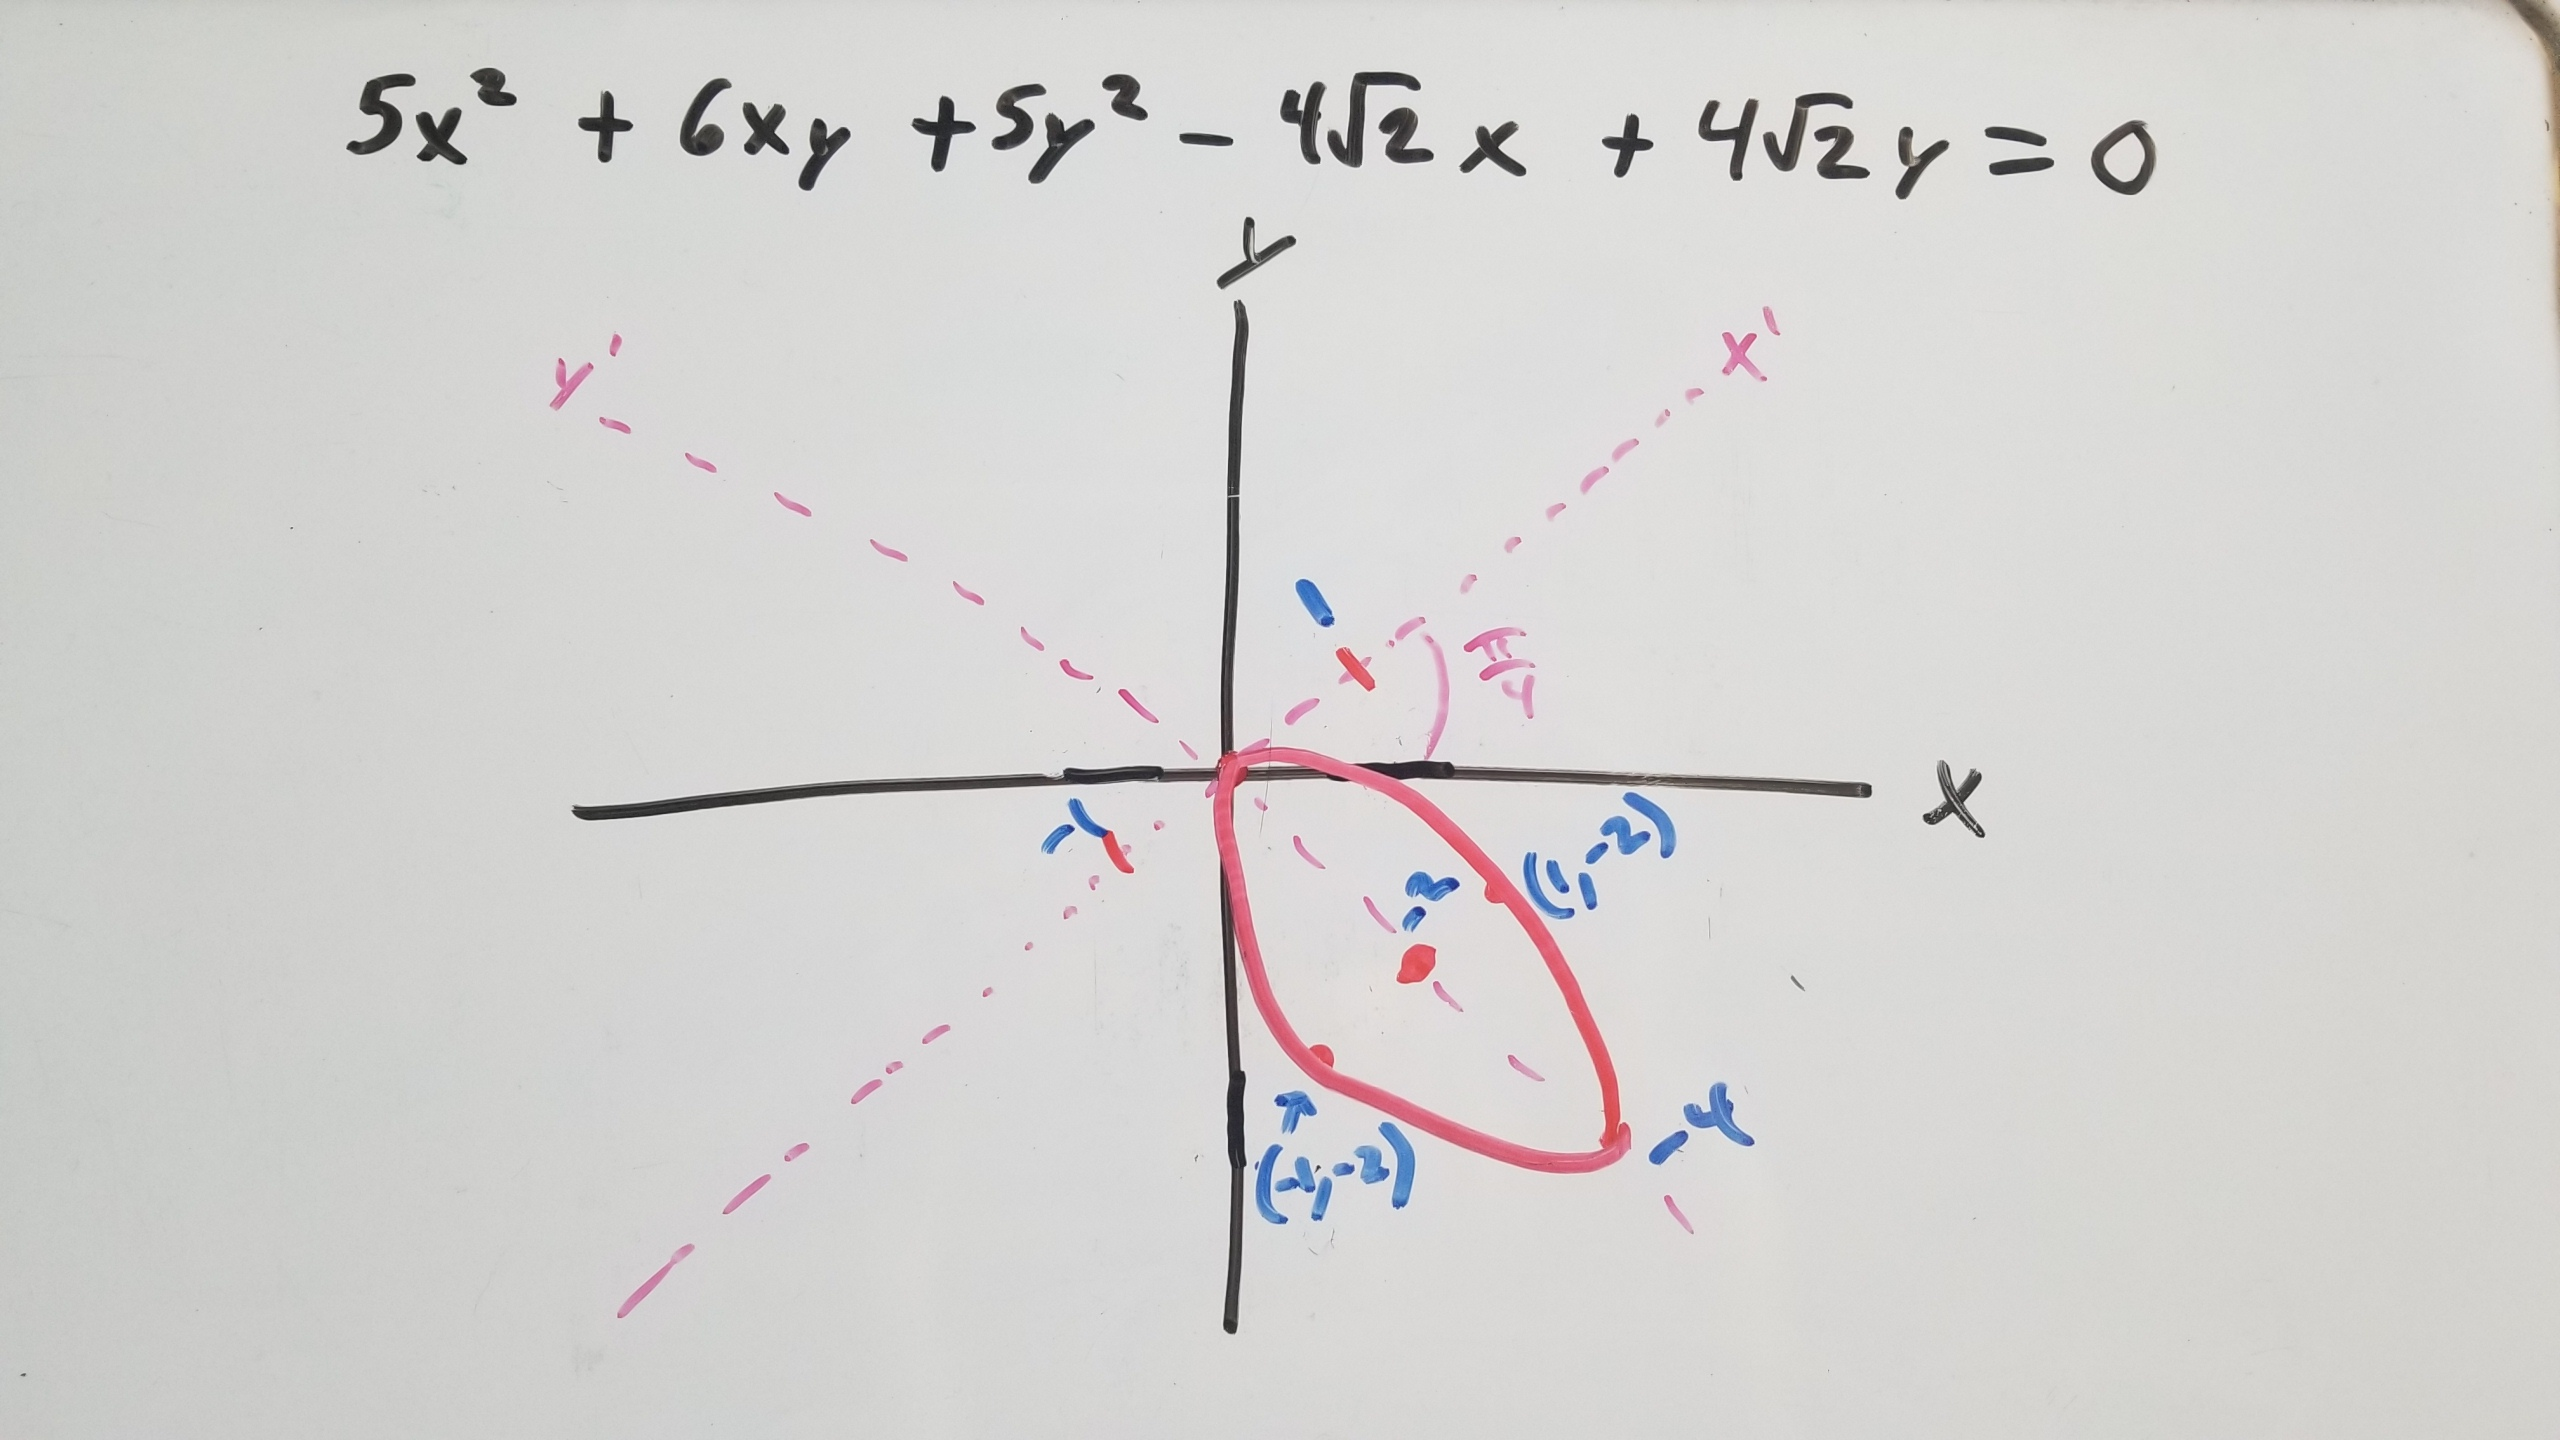
\includegraphics[scale=0.17]{images/11.6_pr_3.jpg}
\end{solution}